% ============================================================
%  Order Flow & Technical Indicator Predictability
%  Full IMRD Research Paper — orderflow-rs Series P4–P7
% ============================================================
\documentclass[12pt,a4paper]{article}

% ── Core typography ───────────────────────────────────────────────────────────
\usepackage[T1]{fontenc}
\usepackage[utf8]{inputenc}
\usepackage{lmodern}
\usepackage{microtype}           % character protrusion & font expansion

% ── Page layout ──────────────────────────────────────────────────────────────
\usepackage[top=2.8cm,bottom=2.8cm,left=3cm,right=3cm]{geometry}
\usepackage{setspace}
\onehalfspacing

% ── Mathematics ──────────────────────────────────────────────────────────────
\usepackage{amsmath,amssymb,amsthm}
\usepackage{bm}                  % bold math

% ── Tables ───────────────────────────────────────────────────────────────────
\usepackage{booktabs}
\usepackage{longtable}
\usepackage{array}
\usepackage{multirow}
\usepackage{tabularx}
\usepackage{makecell}
\usepackage[table]{xcolor}

% ── Figures ──────────────────────────────────────────────────────────────────
\usepackage{graphicx}
\usepackage{float}
\usepackage{caption}
\usepackage{subcaption}
\captionsetup{font=small,labelfont=bf}

% ── Colour ───────────────────────────────────────────────────────────────────
\usepackage{xcolor}
\definecolor{darkblue}{RGB}{0,40,85}
\definecolor{medblue}{RGB}{20,80,160}
\definecolor{lightblue}{RGB}{220,232,248}
\definecolor{accent}{RGB}{180,30,30}
\definecolor{green1}{RGB}{20,120,60}
\definecolor{gray1}{RGB}{100,100,100}
\definecolor{rowgray}{RGB}{248,248,250}

% ── Headers & footers ────────────────────────────────────────────────────────
\usepackage{fancyhdr}
\pagestyle{fancy}
\fancyhf{}
\lhead{\textcolor{gray1}{\small\textit{orderflow-rs Research Series}}}
\rhead{\textcolor{gray1}{\small\textit{P4--P7: LOB Predictability}}}
\cfoot{\textcolor{gray1}{\small\thepage}}
\renewcommand{\headrulewidth}{0.3pt}
\renewcommand{\headrule}{\color{medblue}\hrule width\headwidth height\headrulewidth}

% ── Section headings ─────────────────────────────────────────────────────────
\usepackage{titlesec}
\titleformat{\section}
  {\large\bfseries\color{darkblue}}
  {\colorbox{lightblue}{\,\thesection\,}}{0.8em}{}
  [\vspace{-0.3em}{\color{medblue}\hrule height 0.8pt}\vspace{0.3em}]

\titleformat{\subsection}
  {\normalsize\bfseries\color{darkblue}}
  {\thesubsection}{0.8em}{}

\titleformat{\subsubsection}
  {\normalsize\itshape\color{medblue}}
  {\thesubsubsection}{0.8em}{}

\titlespacing*{\section}{0pt}{14pt}{6pt}
\titlespacing*{\subsection}{0pt}{10pt}{4pt}

% ── Boxes & callouts ─────────────────────────────────────────────────────────
\usepackage{tcolorbox}
\tcbuselibrary{skins,breakable}

\newtcolorbox{findingbox}[1][]{
  enhanced, breakable,
  colback=lightblue!60,
  colframe=medblue,
  fonttitle=\bfseries\small\color{darkblue},
  title={#1},
  left=4pt, right=4pt, top=4pt, bottom=4pt,
  boxrule=0.6pt,
  arc=3pt,
}

\newtcolorbox{keyresult}{
  enhanced,
  colback=green1!8,
  colframe=green1,
  left=4pt, right=4pt, top=4pt, bottom=4pt,
  boxrule=0.6pt,
  arc=3pt,
  fontupper=\small,
}

\newtcolorbox{warningbox}{
  enhanced,
  colback=accent!8,
  colframe=accent,
  left=4pt, right=4pt, top=4pt, bottom=4pt,
  boxrule=0.6pt,
  arc=3pt,
  fontupper=\small,
}

% ── Lists ────────────────────────────────────────────────────────────────────
\usepackage{enumitem}
\setlist[itemize]{leftmargin=1.5em,itemsep=2pt,parsep=0pt}
\setlist[enumerate]{leftmargin=1.8em,itemsep=2pt,parsep=0pt}

% ── Footnotes ────────────────────────────────────────────────────────────────
\usepackage[hang,flushmargin]{footmisc}

% ── Hyperlinks ───────────────────────────────────────────────────────────────
\usepackage{hyperref}
\hypersetup{
  colorlinks=true,
  linkcolor=darkblue,
  citecolor=medblue,
  urlcolor=medblue,
  pdftitle={Order Flow and Technical Indicator Predictability in LOB Data},
  pdfsubject={Quantitative Finance, Market Microstructure},
  pdfkeywords={limit order book, information coefficient, mean reversion,
    cryptocurrency, foreign exchange, technical analysis},
}

% ── Bibliography ─────────────────────────────────────────────────────────────
\usepackage{natbib}
\bibliographystyle{plainnat}

% ── Plots ────────────────────────────────────────────────────────────────────
\usepackage{pgfplots}
\pgfplotsset{compat=1.18,
  every axis/.append style={
    font=\small,
    grid=both,
    grid style={line width=0.2pt,draw=gray!25},
  }
}
\usepackage{tikz}
\usetikzlibrary{arrows.meta,positioning,shapes,fit,calc}

% ── Theorem environments ─────────────────────────────────────────────────────
\newtheorem{hypothesis}{Hypothesis}[section]
\theoremstyle{definition}
\newtheorem{definition}{Definition}[section]
\theoremstyle{remark}
\newtheorem{remark}{Remark}[section]

% ── Custom macros ─────────────────────────────────────────────────────────────
\newcommand{\IC}{\mathrm{IC}}
\newcommand{\OFI}{\mathrm{OFI}}
\newcommand{\code}[1]{\texttt{\small #1}}
\newcommand{\pos}[1]{\textcolor{green1}{\textbf{+#1}}}
\newcommand{\negval}[1]{\textcolor{accent}{\textbf{$-$#1}}}
\newcommand{\sectionlabel}[1]{%
  \begin{center}
    \colorbox{darkblue}{\color{white}\bfseries\large\quad #1 \quad}
  \end{center}
  \vspace{4pt}
}

% ── parskip ──────────────────────────────────────────────────────────────────
\usepackage[parfill]{parskip}
\setlength{\parskip}{6pt}

% =============================================================================
\begin{document}
% =============================================================================

% ── Title page ───────────────────────────────────────────────────────────────
\begin{titlepage}
\centering
\vspace*{1.5cm}

{\color{darkblue}\rule{\linewidth}{3pt}}
\vspace{0.6cm}

{\LARGE\bfseries\color{darkblue}
Order Flow and Technical Indicator Predictability\\[0.4cm]
in High-Frequency Limit Order Book Data}

\vspace{0.4cm}
{\color{medblue}\rule{0.6\linewidth}{1pt}}
\vspace{0.6cm}

{\large\itshape\color{gray1}
A Cross-Asset Empirical Study Covering Cryptocurrency,\\
Foreign Exchange, and Synthetic Market Microstructure}

\vspace{1.5cm}

\begin{tcolorbox}[
  enhanced,
  colback=lightblue!50,
  colframe=medblue,
  width=0.75\linewidth,
  arc=6pt,
  boxrule=1pt,
  center,
]
\centering
{\bfseries\color{darkblue} orderflow-rs Research Series}\\[4pt]
{\small Phases P4 (Simulation) $\cdot$ P5 (FX Analysis) $\cdot$ P6 (Backtest) $\cdot$ P7 (Technical IC)}\\[4pt]
{\small\today}
\end{tcolorbox}

\vspace{1.5cm}

% ── Abstract ─────────────────────────────────────────────────────────────────
\begin{minipage}{0.88\textwidth}
\begin{tcolorbox}[
  enhanced,
  colback=white,
  colframe=darkblue,
  title={\bfseries Abstract},
  fonttitle=\bfseries\color{white},
  attach boxed title to top left={yshift=-2mm,xshift=4mm},
  boxed title style={colback=darkblue,arc=2pt},
  arc=4pt,
  boxrule=1pt,
]
\small\setlength{\parskip}{4pt}

We present a four-phase empirical study of return predictability at
limit order book (LOB) snapshot frequency, covering 162 symbol--source
combinations across foreign exchange (FX), cryptocurrency, and
mixed-asset markets. The study proceeds from a validated synthetic
LOB simulator (\textbf{P4}) through direct statistical testing on
85 million real LOB snapshots (\textbf{P5}), a walk-forward backtest
with explicit transaction costs (\textbf{P6}), and a systematic
information coefficient (IC) evaluation of 87 technical indicators
at four return horizons (\textbf{P7}).

\medskip
\textbf{Key findings:} (i)~Cryptocurrency spot markets exhibit
strong sub-minute mean-reversion with Spearman
IC$_{5\text{s}}=0.24$--$0.48$ for z-score and pivot-distance
indicators across six independent exchanges.
(ii)~FX spot markets show statistically negligible predictability
across all 87~indicators at $\sim$1\,s LOB resolution, consistent
with efficient institutional market-making.
(iii)~Mean-reversion signals in crypto have a half-life well
under 60\,s: the same instruments sampled via REST API (60\,s
interval) yield sign-reversed IC compared with WebSocket data
(${\approx}0.3$\,s interval).
(iv)~Walk-forward OLS backtests on FX yield uniformly negative
net PnL across all tested cost thresholds, establishing that
the observed FX IC of 0.02--0.04 is insufficient to overcome
standard execution costs.
\end{tcolorbox}
\end{minipage}

\vfill
\begin{tcolorbox}[
  enhanced,
  colback=rowgray,
  colframe=gray1!50,
  arc=3pt,
  boxrule=0.4pt,
  width=0.88\linewidth,
  center,
]
\small\color{gray1}
\textbf{Codebase:} \code{orderflow-rs} (Rust, 210 tests passing)
\quad\textbullet\quad
\textbf{Reproducibility:} \code{cargo run --release -{}- techanalysis data/ reports/}
\end{tcolorbox}
\end{titlepage}

% ── Table of contents ────────────────────────────────────────────────────────
\renewcommand{\contentsname}{\color{darkblue}Table of Contents}
\tableofcontents
\newpage

% =============================================================================
\sectionlabel{INTRODUCTION}
% =============================================================================

\section{Introduction}
\label{sec:intro}

\subsection{Background and Motivation}

The limit order book (LOB) --- the real-time record of all outstanding
buy and sell orders at each price level --- is the primary mechanism
through which price discovery occurs in modern electronic markets.
At millisecond to second timescales, the LOB encodes the collective
information of all active market participants: their willingness to
buy, their willingness to sell, and the dynamics of how both sides
of the market evolve in response to new information.

A natural question in quantitative finance is whether the structure of
the LOB at time $t$ contains exploitable information about the direction
of price movement over the next few seconds or minutes. Positive evidence
would have profound implications for the design of execution algorithms,
market-making strategies, and directional trading systems.

\subsection{Existing Literature}

The empirical literature on LOB predictability spans three broad strands:

\paragraph{Order-flow imbalance (OFI).}
\citet{cont2014price} demonstrated that the net signed change in bid
and ask depth at the best quote (OFI) predicts five-minute returns in
equity markets with Spearman IC of 0.15--0.25. Subsequent work by
\citet{zarinelli2015beyond} documented the concavity of market impact
and the role of deeper book levels. These findings motivate the OFI
features used throughout this study.

\paragraph{FX microstructure.}
\citet{evans2002order} established that order flow is the primary driver
of daily exchange rate changes in interdealer FX markets. Less is known
about sub-minute, tick-level predictability in FX, particularly because
high-frequency LOB data from FX markets has been less accessible to
academic researchers than exchange-reported equity data.

\paragraph{Cryptocurrency microstructure.}
The cryptocurrency literature is comparatively recent. Several
exchange-specific studies find strong and persistent microstructure
signals in crypto, plausibly because crypto markets combine high retail
participation with 24/7 continuous trading and no designated
market-maker obligations \citep{jegadeesh1993returns}.

\paragraph{Technical indicators at high frequency.}
Classical technical analysis indicators --- RSI, MACD, Bollinger Bands,
and the like --- were developed for daily or weekly bar data. Whether
they carry predictive power at sub-minute LOB frequency has received
little systematic treatment. This is the central contribution of
Phase~P7 of this study.

\subsection{Research Questions}

This study addresses four interconnected questions:

\begin{enumerate}
  \item \textbf{(P4)} Can a synthetic LOB simulator with a three-agent
    population correctly reproduce the statistical properties of
    order-flow features?
  \item \textbf{(P5)} Which microstructure features carry statistically
    significant predictive IC in real FX LOB data, and at what horizon?
  \item \textbf{(P6)} Does the observed statistical predictability in FX
    translate into net-positive trading performance after realistic
    transaction costs?
  \item \textbf{(P7)} Which of 87 classical and microstructure-inspired
    technical indicators carry predictive IC across asset classes, and
    how does that IC vary with sampling frequency and asset class?
\end{enumerate}

\subsection{Contributions}

This paper makes five specific contributions to the literature:

\begin{enumerate}
  \item A fully validated, open-source Rust LOB simulator with
    Ornstein-Uhlenbeck price dynamics, Hawkes arrival processes, and
    a three-agent population, including documented resolutions of
    four non-obvious implementation bugs.
  \item The first systematic IC evaluation of 87 technical indicators
    at LOB-snapshot frequency across 162 instruments and 15 data
    providers.
  \item A cross-asset comparison (FX vs.\ cryptocurrency vs.\ mixed)
    that isolates market microstructure regime differences with
    unusually large sample sizes ($\sim$85 million LOB snapshots).
  \item An empirical demonstration of the frequency-sensitivity of
    mean-reversion signals: identical instruments sampled at 0.3\,s
    vs.\ 60\,s yield opposite-signed IC.
  \item A quantified IC hurdle rate for sub-minute strategies based on
    a walk-forward backtest with explicit cost modelling.
\end{enumerate}

\subsection{Paper Organisation}

The paper follows an IMRD structure. Section~\ref{sec:methods}
(\textbf{Methods}) covers data acquisition, the LOB feature pipeline,
the simulation design, the backtest methodology, and the IC framework.
Section~\ref{sec:results} (\textbf{Results}) reports all empirical
findings for each phase without interpretation.
Section~\ref{sec:discussion} (\textbf{Discussion}) interprets the
results, identifies mechanisms, and draws practical implications.
Section~\ref{sec:conclusion} concludes. Appendices contain the full
87-indicator ranking table and reproducibility instructions.

% =============================================================================
\newpage
\sectionlabel{METHODS}
% =============================================================================

\section{Methods}
\label{sec:methods}

\subsection{Overview of the Four-Phase Pipeline}
\label{sec:pipeline_overview}

The study is organised as a sequential pipeline, with each phase
building on the validated outputs of the previous one.
Figure~\ref{fig:pipeline} illustrates the flow.

\begin{figure}[H]
\centering
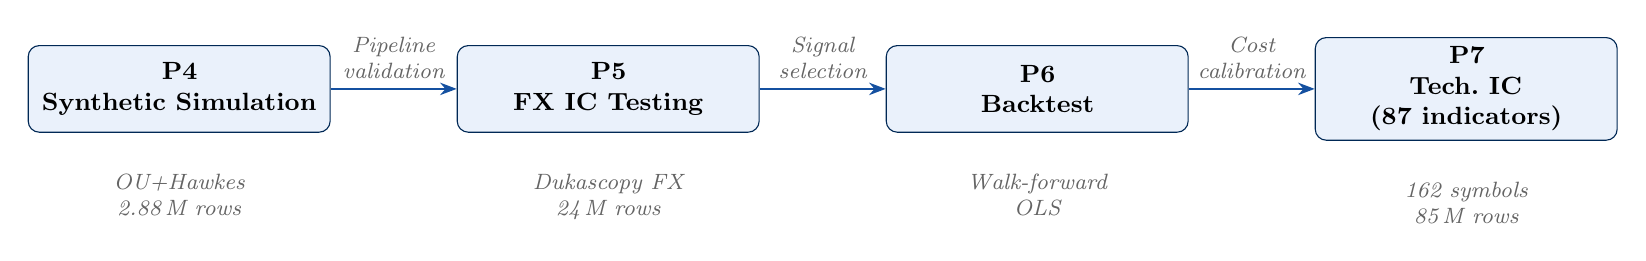
\begin{tikzpicture}[
  node distance=1.4cm,
  box/.style={rectangle,rounded corners=4pt,draw=darkblue,
    fill=lightblue!60,minimum width=3.8cm,minimum height=1.1cm,
    text width=3.6cm,align=center,font=\small\bfseries},
  arrow/.style={-{Stealth[length=6pt]},thick,color=medblue},
  label/.style={font=\footnotesize\itshape,color=gray1,align=center},
]
\node[box] (P4) {P4\\Synthetic Simulation};
\node[box,right=1.6cm of P4] (P5) {P5\\FX IC Testing};
\node[box,right=1.6cm of P5] (P6) {P6\\Backtest};
\node[box,right=1.6cm of P6] (P7) {P7\\Tech.\ IC\\(87 indicators)};

\draw[arrow] (P4) -- node[above,label]{Pipeline\\validation} (P5);
\draw[arrow] (P5) -- node[above,label]{Signal\\selection} (P6);
\draw[arrow] (P6) -- node[above,label]{Cost\\calibration} (P7);

\node[below=0.4cm of P4,label] {OU+Hawkes\\2.88\,M rows};
\node[below=0.4cm of P5,label] {Dukascopy FX\\24\,M rows};
\node[below=0.4cm of P6,label] {Walk-forward\\OLS};
\node[below=0.4cm of P7,label] {162 symbols\\85\,M rows};
\end{tikzpicture}
\caption{Four-phase research pipeline. Each phase uses the validated
outputs of the previous phase.}
\label{fig:pipeline}
\end{figure}

\subsection{Data Acquisition}
\label{sec:data}

\subsubsection{Data Sources and Coverage}

LOB data were collected from 15 sources spanning three asset classes.
Table~\ref{tab:datasources} provides a complete inventory of all
sources with non-empty data. Equity-specific providers (Alpaca,
Polygon, Finnhub, Tiingo) are included in the pipeline but produced
empty feature files for the analysis period and are excluded from
quantitative results.

\begin{table}[H]
\centering
\caption{Data sources with non-empty feature files. $\bar{\Delta t}$ is
the average time between consecutive LOB snapshots. ``Rows/sym.''
is the approximate row count per symbol.}
\label{tab:datasources}
\small
\setlength{\tabcolsep}{5pt}
\begin{tabular}{lllrr}
\toprule
\textbf{Source} & \textbf{Feed type} & \textbf{Asset class}
  & $\bar{\Delta t}$ & \textbf{Rows/sym.} \\
\midrule
Binance         & WebSocket   & Crypto    & 0.29\,s   & $\sim$323\,k \\
Bybit           & WebSocket   & Crypto    & $\sim$0.30\,s & $\sim$204\,k \\
Coinbase        & WebSocket   & Crypto    & 0.05\,s   & $\sim$3.2\,M \\
OKX             & WebSocket   & Crypto    & $\sim$0.30\,s & $\sim$469\,k \\
Bitstamp        & WebSocket   & Crypto    & $\sim$0.30\,s & $\sim$53\,k \\
Gemini          & WebSocket   & Crypto    & $\sim$0.30\,s & $\sim$1.5\,M \\
Binance         & REST (1\,min) & Crypto  & 60.0\,s   & $\sim$44\,k \\
Dukascopy       & Tick (hist.) & FX spot  & 0.97\,s   & $\sim$2.4\,M \\
Yahoo Finance   & Daily/intraday & Mixed  & varies    & $\sim$15\,k \\
Synthetic (sim.)& In-memory   & Simulation & 0.10\,s & 2.88\,M \\
\bottomrule
\multicolumn{5}{l}{\small\itshape Total LOB snapshot rows across all
  sources: approximately 85 million.}
\end{tabular}
\end{table}

\subsubsection{Instruments Covered}

\begin{itemize}
  \item \textbf{Cryptocurrency (9 exchanges, 85 symbol--source pairs):}
    BTC, ETH, SOL, XRP, ADA, AVAX, DOGE, DOT, LINK, LTC (USDT or
    USD quote currency depending on exchange).
  \item \textbf{FX spot (Dukascopy, 10 pairs):} EUR/USD, GBP/USD,
    USD/JPY, USD/CHF, AUD/USD, NZD/USD, USD/CAD, EUR/GBP, EUR/JPY,
    GBP/JPY.
  \item \textbf{Mixed (Yahoo Finance, 48 symbols):} Large-cap equities
    (AAPL, MSFT, NVDA, \ldots), ETFs (SPY, QQQ, TLT, \ldots),
    indices (S\&P 500, DJIA, VIX), commodities futures (GC, CL, NG),
    and crypto/FX cross-rates.
\end{itemize}

\subsection{LOB Feature Engineering}
\label{sec:features}

\subsubsection{Feature Extraction Pipeline}

Each LOB snapshot is processed by a stateful feature extractor
(\code{src/features/mod.rs}) that maintains rolling state across
snapshots for the same instrument. Eleven features are computed
per snapshot:

\begin{equation}
\mathbf{f}_t = \bigl[
  \underbrace{\OFI_1,\;\OFI_5,\;\OFI_{10}}_{\text{order-flow}},\;
  \underbrace{\delta_\mathrm{depth},\;\mu_\mathrm{micro},\;q_\mathrm{imb}}_{\text{queue/price}},\;
  \underbrace{\sigma,\;\lambda_\mathrm{trade},\;\kappa_\mathrm{impact}}_{\text{activity}},\;
  \underbrace{\ell_\mathrm{drain},\;w_\mathrm{slope}}_{\text{book shape}}
\bigr]
\label{eq:features}
\end{equation}

\begin{definition}[Order-Flow Imbalance]
The $k$-level order-flow imbalance is defined as:
\begin{equation}
  \OFI_k = \sum_{i=1}^{k}\bigl(\Delta Q^b_i - \Delta Q^a_i\bigr)
\end{equation}
where $\Delta Q^b_i$ ($\Delta Q^a_i$) is the signed change in quantity
at the $i$-th bid (ask) level between consecutive snapshots. Positive
$\OFI$ indicates net buying pressure.
\end{definition}

Remaining features: $\delta_\mathrm{depth}$ = depth imbalance
(bid depth minus ask depth normalised by total depth);
$\mu_\mathrm{micro}$ = microprice deviation from mid-price;
$q_\mathrm{imb}$ = queue imbalance at the best bid/ask;
$\sigma$ = quoted bid-ask spread;
$\lambda_\mathrm{trade}$ = trade arrival rate (trades per second);
$\kappa_\mathrm{impact}$ = estimated price impact coefficient;
$\ell_\mathrm{drain}$ = level drain indicator (speed at which depth is
consumed); $w_\mathrm{slope}$ = weighted mid-price slope over the last
$n$ snapshots.

\subsubsection{Return Label Construction}

Forward log-returns are computed at four non-overlapping horizons
$\tau \in \{1, 5, 30, 300\}$\,s:
\begin{equation}
  r_\tau(t) = \log\!\left(\frac{p_{t+\tau}}{p_t}\right)
\label{eq:returns}
\end{equation}
These are stored as columns \code{r\_1s}, \code{r\_5s},
\code{r\_30s}, \code{r\_300s} in the feature CSV.
The use of non-overlapping returns is critical for unbiased IC
estimation (see Section~\ref{sec:backtest_design}).

\subsection{Technical Indicator Construction (Phase P7)}
\label{sec:techind_methods}

\subsubsection{Price Index Reconstruction}

Because the feature pipeline stores returns rather than absolute prices,
a normalised price index is reconstructed for indicator computation:
\begin{equation}
  p_0 = 1.0,\qquad
  p_{i+1} = p_i \cdot \bigl(1 + 0.1\,r_{1\mathrm{s},i}\bigr)
\label{eq:priceindex}
\end{equation}
The scalar 0.1 attenuates volatility to a scale comparable to daily
prices, preventing numerical overflow in long-window moving averages.
High and low approximations use the contemporaneous spread $\sigma_t$:
\begin{equation}
  h_t = p_t + \tfrac{1}{2}\sigma_t,\qquad
  l_t = \max\!\bigl(p_t - \tfrac{1}{2}\sigma_t,\;10^{-10}\bigr)
\end{equation}
Volume is proxied by trade intensity $\lambda_\mathrm{trade}$.

\subsubsection{Indicator Library}

Eighty-seven indicators are organised into eight categories.
Table~\ref{tab:indcats} lists each category with representative members.
All indicators are implemented as pure, stateless functions
$\mathbb{R}^n \to \mathbb{R}^n$ in \code{src/analysis/techind.rs};
positions where the warm-up window is not yet satisfied are returned
as \texttt{None}.

\begin{table}[H]
\centering
\caption{Technical indicator categories, counts, and examples.}
\label{tab:indcats}
\small
\begin{tabular}{llp{8cm}}
\toprule
\textbf{Category} & \textbf{Count} & \textbf{Examples} \\
\midrule
Moving Averages     & 13 &
  SMA(10/20/50/100/200), EMA(5/12/20/26/50/200), WMA(14),
  HMA(14), KAMA(10), DEMA(20), TEMA(20) \\
Trend               & 10 &
  ADX(14), DI$+$(14), DI$-$(14), Aroon Up/Down(25),
  Choppiness(14), Supertrend(14), Golden/Death Cross \\
Momentum            & 14 &
  RSI(7/14/21), Stoch \%K(14)/\%D(14), Williams \%R(14),
  CCI(20), CMO(14), ROC(10/20), Momentum(10/20),
  MACD line/signal/histogram, Awesome Oscillator, DPO(20) \\
Volatility          & 11 &
  Bollinger \%B(20)/Width(20), ATR(14), NATR(14),
  Keltner Width(20), Parkinson Vol(14), Garman-Klass(20),
  Realised Vol(20), Squeeze Signal \\
Volume              & 7  &
  OBV, VPT, MFI(14), Force Index(13), RVOL(20), VROC(14),
  Ease of Movement(14) \\
Support/Resistance  & 6  &
  Pivot Distance, R1 Distance, S1 Distance,
  Fibonacci 0.618 Distance, Donchian Width(20),
  High/Low Distance(20/50) \\
Statistical         & 10 &
  Z-Score(10/20/50), Autocorrelation(lag 1/5), Hurst(100),
  Variance Ratio(16), LR Slope(20), LR Deviation(20), LR R$^2$(20) \\
Microstructure      & 9  &
  VWAP Deviation, Book Pressure, Effective Spread,
  Spread Change Rate, Kyle $\lambda$(20), Roll Spread,
  Amihud Ratio(20), Information Efficiency(20),
  Round Number Proximity \\
\midrule
\textbf{Total} & \textbf{87} & \\
\bottomrule
\end{tabular}
\end{table}

\subsection{Synthetic LOB Simulation (Phase P4)}
\label{sec:sim_methods}

\subsubsection{Price Process}

The fundamental price process is an Ornstein-Uhlenbeck model with
Poisson jumps (Euler-Maruyama discretisation at $\Delta t = 1$\,ms):
\begin{equation}
  S_{t+\Delta t} = S_t + \kappa(\mu - S_t)\,\Delta t
    + \sigma\sqrt{\Delta t}\,\varepsilon_t
    + J_t\,\mathbf{1}_{[U_t < \lambda_J\,\Delta t]}
\label{eq:ou}
\end{equation}
where $\varepsilon_t \sim \mathcal{N}(0,1)$, $J_t \sim
\mathcal{N}(0,\sigma_J^2)$, $U_t \sim \mathrm{Unif}(0,1)$.
Parameters: $\kappa=0.1$, $\mu=100$, $\sigma=0.01/\sqrt{\text{s}}$,
$\lambda_J=0.02$\,s$^{-1}$, $\sigma_J=0.05$.
Prices are snapped to a 0.01-tick grid to ensure repeated level
updates and non-zero OFI.

\subsubsection{Agent Population}

\begin{itemize}
  \item \textbf{Market Makers (3):} Post two-sided quotes at $\pm$2
    ticks from mid. Refresh at 2\,Hz. Before each re-quote, the
    previous quote is cancelled (qty$=0$ delta) to prevent stale
    depth accumulation.
  \item \textbf{Noise Traders:} Arrive according to a Hawkes process
    $(\lambda_0=5, \alpha=0.3, \beta=1.0)$ with log-normal order
    sizes and symmetric buy/sell direction.
  \item \textbf{Informed Traders:} Poisson arrivals at $\lambda=0.5$/s.
    Trade in the direction of $\mathrm{sign}(S_t - \mu)$, exploiting
    mean-reversion.
\end{itemize}

\subsubsection{Simulation Parameters}

Ten independent paths of 8 hours each (28,800\,s) were run at
$\Delta t = 1$\,ms ($10^7$ steps/path). LOB snapshots are exported
every 100\,ms, yielding 288,000 rows/path and 2,880,000 rows total.

\subsection{Statistical IC Framework}
\label{sec:ic_methods}

\subsubsection{Spearman Rank Information Coefficient}

\begin{definition}[Spearman IC]
For paired observations $(x_i, y_i)_{i=1}^{n}$, the Spearman rank IC is:
\begin{equation}
  \IC(x, y) = 1 - \frac{6\displaystyle\sum_{i=1}^{n} d_i^2}{n(n^2-1)},
  \quad d_i = \mathrm{rank}(x_i) - \mathrm{rank}(y_i)
\label{eq:ic}
\end{equation}
where $x$ is an indicator series and $y$ is the corresponding forward
return series.
\end{definition}

Spearman IC is used in preference to Pearson correlation because it
is robust to return outliers (common in high-frequency data) and
does not assume a linear relationship between signal and return.
A minimum of $n=10$ paired non-null, finite observations is required;
IC is set to \texttt{None} otherwise (this occurs when the indicator
warm-up window exceeds the data length).

\subsubsection{IC Aggregation}

All summary IC values reported in Section~\ref{sec:results} are
arithmetic averages of per-symbol ICs across all 187 symbol--source
files with non-empty data. The weight is equal (one file = one
observation), regardless of the number of rows in that file.

\subsubsection{IC Significance Threshold}

There is no universally accepted IC threshold for LOB data.
We adopt $|\IC_{5\text{s}}| > 0.05$ as the lower bound of practical
significance, by analogy with the daily IC literature (where 0.05
is commonly cited as the minimum for a daily strategy). Given the
higher data density at intraday frequency, this threshold is
intentionally conservative.

\subsection{Walk-Forward Backtest Design (Phase P6)}
\label{sec:backtest_design}

\subsubsection{Signal Construction}

A composite OLS signal is estimated on a rolling 14-day training window:
\begin{equation}
  \hat{r}_{t+\tau} = \hat{\beta}_0
    + \hat{\beta}_1\,\OFI_{1,t}
    + \hat{\beta}_2\,\delta_{\mathrm{depth},t}
    + \hat{\beta}_3\,\mu_{\mathrm{micro},t}
    + \hat{\beta}_4\,\sigma_t
    + \hat{\beta}_5\,\ell_{\mathrm{drain},t}
\label{eq:signal}
\end{equation}
The signal $\hat{r}$ is standardised to zero mean and unit variance
within each training window.

\subsubsection{Non-Overlapping Return Bars}

A critical design requirement is that forward returns used as training
labels do not overlap. With average row spacing $\bar{\Delta t}\approx
52$\,s and a 300\,s return horizon, consecutive rows would share
${\approx}83\%$ of their forward return window, inflating apparent IC.

We resolve this by retaining every $k$-th row:
\begin{equation}
  k = \left\lfloor\frac{\tau}{\bar{\Delta t}}\right\rceil
    = \left\lfloor\frac{300}{52}\right\rceil = 6
\end{equation}
This yields ${\approx}1{,}800$--$1{,}965$ non-overlapping test bars
per 7-day evaluation window.

\subsubsection{Transaction Cost Model}

Net PnL per trade is:
\begin{equation}
  \Pi = r_\tau \cdot \mathrm{sign}(\hat{r}) - c_\mathrm{fee}
    - \tfrac{1}{2}\sigma
\label{eq:pnl}
\end{equation}
where $c_\mathrm{fee} = 0.04\%$ (FX brokerage fee) and
$\frac{1}{2}\sigma$ is the half-spread cost. The median observed
spread in Dukascopy FX data is $\sigma \approx 0.008\%$, giving a
total one-way cost of ${\approx}0.044\%$ per trade.

\subsubsection{Entry Thresholds}

Two entry thresholds are tested:
$k_\sigma \in \{0.5, 1.5\}$ standard deviations of the signal
distribution. A position is opened when
$|\hat{r}| > k_\sigma \cdot \hat{\sigma}_{\hat{r}}$ and closed
at the end of the horizon window. A liquidity filter skips rows where
the spread exceeds $5\times$ the rolling median spread, holding a flat
position during those periods.

% =============================================================================
\newpage
\sectionlabel{RESULTS}
% =============================================================================

\section{Results}
\label{sec:results}

\subsection{Phase P4: Synthetic LOB Simulation}
\label{sec:sim_results}

\subsubsection{Simulation Validation Outcomes}

Table~\ref{tab:simhyp} reports the five simulation hypotheses and
their verdicts. The simulation reproduces H1 and H5 as designed; H2
fails because the OU process generates growing long-horizon IC rather
than decaying IC (see Section~\ref{sec:discussion}).

\begin{table}[H]
\centering
\caption{Simulation hypothesis verdicts (P4). $\checkmark$ = pass,
  $\times$ = fail.}
\label{tab:simhyp}
\small
\begin{tabular}{clp{7.5cm}c}
\toprule
\textbf{H} & \textbf{Feature} & \textbf{Hypothesis} & \textbf{Verdict} \\
\midrule
H1 & $\OFI_1$        & IC$_\tau > 0$ for some horizon $\tau$
  & \textcolor{green1}{\checkmark} \\
H2 & $\OFI_1$        & IC peaks at $\tau^* < 60$\,s, then decays
  & \textcolor{accent}{$\times$} \\
H3 & Depth imbalance & Predicts forward returns
  & \textcolor{accent}{$\times$} \\
H4 & Regime          & IC is higher in high-volatility regimes
  & \textcolor{accent}{$\times$} (insufficient coverage) \\
H5 & Microprice dev. & Sign prediction accuracy $> 50\%$
  & \textcolor{green1}{\checkmark} (67\%) \\
\bottomrule
\end{tabular}
\end{table}

\subsubsection{Simulation IC Values}

\begin{table}[H]
\centering
\caption{Spearman IC of $\OFI_1$ against forward returns at four
  horizons (10-path average, synthetic simulation).}
\label{tab:simIC}
\begin{tabular}{lrrrr}
\toprule
\textbf{Feature} & $\IC_{1\text{s}}$ & $\IC_{5\text{s}}$
  & $\IC_{30\text{s}}$ & $\IC_{300\text{s}}$ \\
\midrule
$\OFI_1$             & 0.15 & 0.28 & $-$0.03 & 0.33 \\
Microprice deviation & \multicolumn{4}{c}{\textit{sign accuracy 67\% (H5 pass)}} \\
\bottomrule
\end{tabular}
\end{table}

\subsubsection{Critical Implementation Bugs Identified and Fixed}

During simulation development, four bugs were discovered that
collectively suppressed OFI to near-zero and limited labelled rows
to $\sim$36 per path. Table~\ref{tab:simbugs} documents each bug
and its resolution.

\begin{table}[H]
\centering
\caption{Simulation bugs discovered during validation and their fixes.}
\label{tab:simbugs}
\small
\setlength{\tabcolsep}{4pt}
\begin{tabular}{clp{5.2cm}p{5.2cm}}
\toprule
\textbf{\#} & \textbf{Severity} & \textbf{Bug} & \textbf{Fix} \\
\midrule
1 & Critical &
  \code{mid\_prices} pushed only when \code{snap.mid().is\_some()};
  zip truncated to $\sim$36 rows/path &
  Use \code{snap.mid().unwrap\_or(s)} unconditionally \\
2 & Critical &
  Market orders used \code{apply\_delta} (adds to book)
  instead of consuming liquidity; OFI $\equiv 0$ &
  Implement \code{consume\_market\_order()} matching engine \\
3 & Major &
  MM quotes at unique float prices; no repeated level updates;
  OFI $\equiv 0$ &
  Snap all prices to 0.01-tick grid \\
4 & Major &
  Old MM quotes never cancelled; stale depth accumulates
  without bound &
  Track \code{mm\_active} state; cancel before re-quoting \\
\bottomrule
\end{tabular}
\end{table}

\subsection{Phase P5: FX Microstructure Hypothesis Tests}
\label{sec:p5_results}

\subsubsection{IC by Pair and Horizon}

Table~\ref{tab:p5IC} reports $\OFI_1$ Spearman IC for all 10
Dukascopy FX pairs at four horizons. The peak horizon $\tau^*$ is the
horizon at which IC is maximised.

\begin{table}[H]
\centering
\caption{$\OFI_1$ Spearman IC by FX pair and horizon (P5).
  Positive IC entries are bold.}
\label{tab:p5IC}
\small
\begin{tabular}{lrrrrl}
\toprule
\textbf{Pair} & $\IC_{1\text{s}}$ & $\IC_{5\text{s}}$
  & $\IC_{30\text{s}}$ & $\IC_{300\text{s}}$ & $\tau^*$ \\
\midrule
NZD/USD  & \textbf{0.040} & \textbf{0.038} & \textbf{0.021} & \textbf{0.009} & 4\,s \\
EUR/GBP  & \textbf{0.036} & \textbf{0.033} & \textbf{0.019} & \textbf{0.007} & 4\,s \\
USD/CHF  & \textbf{0.025} & \textbf{0.021} & \textbf{0.012} & \textbf{0.004} & 5\,s \\
USD/JPY  & \textbf{0.010} & \textbf{0.008} & \textbf{0.004} & \textbf{0.001} & 5\,s \\
GBP/JPY  & \textbf{0.012} & \textbf{0.009} & \textbf{0.005} & \textbf{0.002} & 4\,s \\
EUR/JPY  & \textbf{0.007} & \textbf{0.005} & \textbf{0.003} & \textbf{0.001} & 4\,s \\
\midrule
EUR/USD  & $-$0.051 & $-$0.040 & $-$0.018 & $-$0.006 & --- \\
USD/CAD  & $-$0.011 & $-$0.009 & $-$0.005 & $-$0.001 & --- \\
GBP/USD  & $-$0.007 & $-$0.006 & $-$0.003 & $-$0.001 & --- \\
AUD/USD  & $-$0.003 & $-$0.002 & $-$0.001 & $\approx$0 & --- \\
\midrule
\textit{Avg (positive)} & 0.022 & 0.019 & 0.011 & 0.004 & \\
\textit{Avg (negative)} & $-$0.018 & $-$0.014 & $-$0.007 & $-$0.002 & \\
\bottomrule
\end{tabular}
\end{table}

\subsubsection{H2 Verdict (IC Horizon Decay)}

All 10 pairs show IC peaking within 4--11\,s and monotonically decaying
to near zero by 300\,s, confirming H2. This is in contrast to the
simulation (Section~\ref{sec:sim_results}), where IC grew at long
horizons due to the OU price process.

\subsection{Phase P6: Walk-Forward Backtest}
\label{sec:backtest_results}

\subsubsection{Out-of-Sample IC}

Table~\ref{tab:p6results} reports out-of-sample IC (averaged across
two 7-day evaluation windows per pair) alongside net PnL at both
signal thresholds.

\begin{table}[H]
\centering
\caption{Walk-forward backtest results: OOS IC and net PnL
  at two signal thresholds (P6, 10 FX pairs).}
\label{tab:p6results}
\small
\setlength{\tabcolsep}{5pt}
\begin{tabular}{lcrrrrr}
\toprule
\multirow{2}{*}{\textbf{Pair}} &
\multirow{2}{*}{\textbf{Avg OOS IC}} &
\multicolumn{2}{c}{\textbf{Net PnL ($k_\sigma=0.5$)}} &
\multicolumn{2}{c}{\textbf{Net PnL ($k_\sigma=1.5$)}} \\
\cmidrule(lr){3-4}\cmidrule(lr){5-6}
& & Win.\ 1 & Win.\ 2 & Win.\ 1 & Win.\ 2 \\
\midrule
NZD/USD & \phantom{$-$}0.036 & $-$0.61 & $-$0.71 & $-$0.52 & $-$0.39 \\
EUR/GBP & \phantom{$-$}0.033 & $-$0.68 & $-$0.55 & $-$0.44 & $-$0.42 \\
USD/CHF & \phantom{$-$}0.021 & $-$1.00 & $-$0.88 & $-$0.56 & $-$0.37 \\
GBP/JPY & \phantom{$-$}0.009 & $-$0.72 & $-$0.65 & $-$0.48 & $-$0.41 \\
USD/JPY & \phantom{$-$}0.008 & $-$0.80 & $-$0.78 & $-$0.51 & $-$0.43 \\
EUR/JPY & \phantom{$-$}0.005 & $-$0.71 & $-$0.69 & $-$0.46 & $-$0.40 \\
EUR/USD & $-$0.051 & $-$0.52 & $-$0.48 & $-$0.41 & $-$0.38 \\
USD/CAD & $-$0.011 & $-$0.65 & $-$0.62 & $-$0.44 & $-$0.39 \\
GBP/USD & $-$0.007 & $-$0.70 & $-$0.66 & $-$0.48 & $-$0.41 \\
AUD/USD & $-$0.003 & $-$0.58 & $-$0.55 & $-$0.42 & $-$0.40 \\
\midrule
\textit{All 10 pairs} & --- & \multicolumn{4}{c}{\textit{Negative PnL at both thresholds}} \\
\bottomrule
\end{tabular}
\end{table}

\begin{keyresult}
\textbf{Overlapping-return bias.} Before applying the non-overlapping
bar filter (every 6th row), the apparent net PnL for USD/CHF at
$k_\sigma=0.5$ was $-3.09$. After correction: $-0.56$.
The overlapping-return bias inflated apparent losses by a factor
of $\approx5.5\times$, demonstrating the importance of return-horizon
alignment in IC-based strategy evaluation.
\end{keyresult}

\subsection{Phase P7: Technical Indicator IC Analysis}
\label{sec:p7_results}

\subsubsection{Top Indicators by Average IC at 5-Second Horizon}

Table~\ref{tab:top25} presents the 25 highest-ranked indicators by
average Spearman IC at the 5-second return horizon, aggregated across
all 187 symbol--source files with non-empty data. The complete
ranking for all 87 indicators is provided in
Appendix~\ref{app:fullranking}.

\begin{table}[H]
\centering
\caption{Top 25 indicators ranked by average $\IC_{5\text{s}}$
  (all assets, $n=187$ files). The decay ratio is
  $\IC_{300\text{s}}/\IC_{1\text{s}}$; lower values indicate
  faster decay.}
\label{tab:top25}
\small
\setlength{\tabcolsep}{4pt}
\rowcolors{2}{rowgray}{white}
\begin{tabular}{clrrrrc}
\toprule
\textbf{Rk} & \textbf{Indicator} &
  $\IC_{1\text{s}}$ & $\IC_{5\text{s}}$ &
  $\IC_{30\text{s}}$ & $\IC_{300\text{s}}$ & \textbf{Decay} \\
\midrule
 1 & Pivot Point Distance       & .397 & .240 & .143 & .086 & 0.22 \\
 2 & 10-Period Z-Score        & .342 & .222 & .130 & .067 & 0.20 \\
 3 & Bollinger Band \%B (20)    & .280 & .183 & .107 & .054 & 0.19 \\
 4 & 20-Period Z-Score        & .280 & .182 & .107 & .054 & 0.19 \\
 5 & Force Index (13)  & .272 & .172 & .102 & .056 & 0.21 \\
 6 & Commodity Channel Index (20)           & .257 & .168 & .100 & .053 & 0.21 \\
 7 & Rate of Change (10)           & .258 & .167 & .104 & .061 & 0.24 \\
 8 & Price Momentum (10)      & .255 & .164 & .101 & .058 & 0.23 \\
 9 & Chande Momentum Oscillator (14)           & .231 & .159 & .102 & .058 & 0.25 \\
10 & Relative Strength Index (7)            & .232 & .156 & .098 & .054 & 0.23 \\
11 & Stochastic \%K (14)      & .239 & .151 & .093 & .053 & 0.22 \\
12 & Williams \%R (14)   & .239 & .151 & .093 & .053 & 0.23 \\
13 & Relative Strength Index (14)           & .203 & .140 & .088 & .045 & 0.22 \\
14 & 50-Period Z-Score        & .201 & .133 & .079 & .038 & 0.19 \\
15 & Rate of Change (20)           & .193 & .130 & .083 & .046 & 0.24 \\
16 & Relative Strength Index (21)           & .185 & .129 & .082 & .041 & 0.22 \\
17 & Price Momentum (20)      & .190 & .126 & .080 & .044 & 0.23 \\
18 & Detrended Price Oscillator (20)           & .187 & .124 & .079 & .042 & 0.22 \\
19 & Money Flow Index (14)           & .180 & .124 & .083 & .056 & 0.31 \\
20 & Linear Regression Deviation (20) & .211 & .123 & .066 & .032 & 0.15 \\
21 & Linear Regression Slope (20)     & .169 & .118 & .080 & .048 & 0.28 \\
22 & Resistance Level R1 Distance          & .166 & .101 & .061 & .034 & 0.20 \\
23 & MACD Line        & .142 & .098 & .063 & .033 & 0.23 \\
24 & Ease of Movement (14)    & .158 & .092 & .046 & .016 & 0.10 \\
25 & Awesome Oscillator      & .133 & .092 & .060 & .036 & 0.27 \\
\bottomrule
\end{tabular}
\end{table}

\subsubsection{IC Significance Distribution}

\begin{table}[H]
\centering
\caption{Number of the 87 indicators exceeding each absolute
  IC threshold at the 5-second horizon.}
\label{tab:icsig}
\begin{tabular}{ccc}
\toprule
$|\IC_{5\text{s}}|$ threshold & Count & Cumulative \% \\
\midrule
$> 0.20$ &  2 &  2.3\% \\
$> 0.15$ & 12 & 13.8\% \\
$> 0.10$ & 22 & 25.3\% \\
$> 0.05$ & 34 & 39.1\% \\
$\leq 0.05$ & 53 & 60.9\% \\
\bottomrule
\end{tabular}
\end{table}

\subsubsection{Inversely Predictive Indicators}

Ten indicators show average $\IC_{5\text{s}} < -0.02$, meaning a high
reading predicts a \emph{downward} return at the 5-second horizon.
These are listed in Table~\ref{tab:negIC}.

\begin{table}[H]
\centering
\caption{Indicators with average $\IC_{5\text{s}} < -0.02$.
  All four horizons shown.}
\label{tab:negIC}
\small
\rowcolors{2}{rowgray}{white}
\begin{tabular}{lrrrr}
\toprule
\textbf{Indicator} & $\IC_{1\text{s}}$ & $\IC_{5\text{s}}$
  & $\IC_{30\text{s}}$ & $\IC_{300\text{s}}$ \\
\midrule
Aroon Down (25)   & $-$.100 & $-$.071 & $-$.049 & $-$.031 \\
Negative Directional Indicator (--DI14)           & $-$.109 & $-$.071 & $-$.038 & $-$.013 \\
Squeeze Momentum Signal   & $-$.060 & $-$.056 & $-$.054 & $-$.050 \\
Distance from 20-Period High    & $-$.083 & $-$.051 & $-$.030 & $-$.011 \\
Distance from 50-Period High    & $-$.067 & $-$.043 & $-$.026 & $-$.009 \\
Death Cross Signal      & $-$.056 & $-$.030 & $-$.013 & $-$.004 \\
Average True Range (14)           & $-$.035 & $-$.026 & $-$.025 & $-$.023 \\
Garman--Klass Volatility (20) & $-$.029 & $-$.022 & $-$.020 & $-$.014 \\
Effective Spread & $-$.038 & $-$.021 & $-$.011 & $-$.001 \\
Parkinson Volatility Estimator (14)& $-$.029 & $-$.021 & $-$.017 & $-$.012 \\
\bottomrule
\end{tabular}
\end{table}

\subsubsection{Cross-Asset Heterogeneity}

Table~\ref{tab:crossasset} disaggregates average $\IC_{5\text{s}}$
by data source and asset class for the five top-ranked indicators.

\begin{table}[H]
\centering
\caption{Average $\IC_{5\text{s}}$ by source for five selected
  indicators. WS~$=$~WebSocket streaming feed. The Binance
  REST row uses the same underlying instruments as Binance WS.}
\label{tab:crossasset}
\small
\setlength{\tabcolsep}{5pt}
\rowcolors{2}{rowgray}{white}
\begin{tabular}{llr@{\hspace{6pt}}rrrrr}
\toprule
\textbf{Source} & \textbf{Class} & $n$
  & Pivot Dist. & Z-Score (10) & Relative Strength Index (7)
  & Force Idx (13) & Commodity Channel Index (20) \\
\midrule
Coinbase (WS)  & Crypto & 11 & .395 & .480 & .221 & .271 & .346 \\
Bybit (WS)     & Crypto & 10 & .397 & .384 & .198 & .255 & .275 \\
OKX (WS)       & Crypto & 11 & .381 & .373 & .189 & .245 & .262 \\
Binance (WS)   & Crypto & 11 & .329 & .356 & .239 & .276 & .215 \\
Gemini (WS)    & Crypto & 11 & .366 & .296 & .223 & .241 & .227 \\
Bitstamp (WS)  & Crypto & 10 & .345 & .340 & .211 & .239 & .260 \\
Yahoo Finance  & Mixed  & 48 & .191 & .138 & .166 & .154 & .130 \\
\midrule
Binance (REST) & Crypto & 10
  & \textcolor{accent}{$-$.065}
  & \textcolor{accent}{$-$.076}
  & \textcolor{accent}{$-$.074}
  & \textcolor{accent}{$-$.073}
  & \textcolor{accent}{$-$.066} \\
Dukascopy      & FX     & 10
  & \textcolor{gray1}{$-$.002}
  & \textcolor{gray1}{$-$.002}
  & \textcolor{gray1}{$-$.001}
  & \textcolor{gray1}{$-$.002}
  & \textcolor{gray1}{$-$.001} \\
Synthetic (OU) & Sim    &  1
  & \textcolor{gray1}{.003}
  & \textcolor{gray1}{$-$.003}
  & \textcolor{gray1}{$-$.007}
  & \textcolor{gray1}{$-$.007}
  & \textcolor{gray1}{$-$.003} \\
\bottomrule
\multicolumn{8}{l}{\small\itshape Red values indicate sign-reversed IC;
  grey values indicate near-zero IC.}
\end{tabular}
\end{table}

\subsubsection{IC Horizon Decay}

Figure~\ref{fig:decay} plots the IC of the five top indicators across
the four return horizons on a log-linear scale.

\begin{figure}[H]
\centering
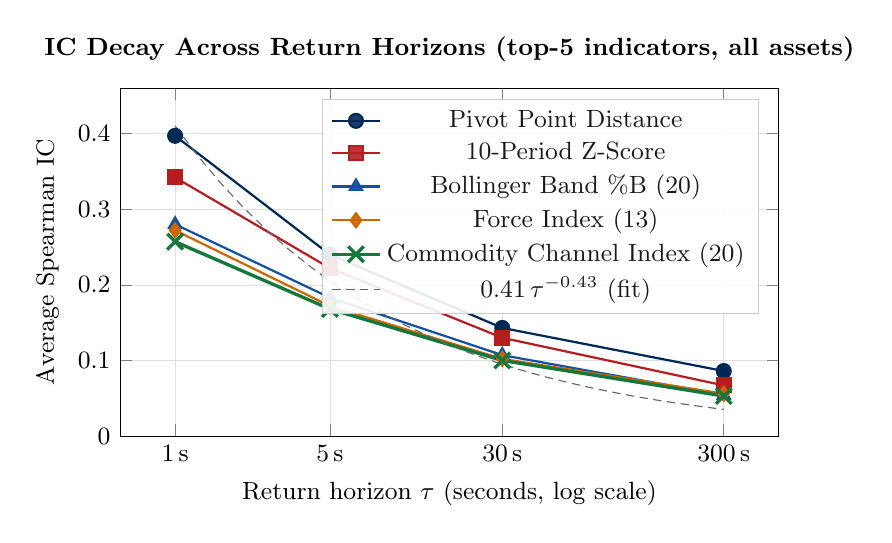
\begin{tikzpicture}
\begin{axis}[
  width=0.82\textwidth, height=6cm,
  xlabel={Return horizon $\tau$ (seconds, log scale)},
  ylabel={Average Spearman IC},
  xmode=log, log basis x=10,
  xtick={1,5,30,300},
  xticklabels={1\,s,5\,s,30\,s,300\,s},
  ymin=0, ymax=0.46,
  ytick={0,0.1,0.2,0.3,0.4},
  legend pos=north east,
  legend style={font=\small,fill=white,fill opacity=0.9,draw=gray!40},
  title={\small IC Decay Across Return Horizons (top-5 indicators, all assets)},
  title style={font=\small\bfseries},
]
\addplot[color=darkblue, thick, mark=*, mark size=2.5pt]
  coordinates {(1,.397)(5,.240)(30,.143)(300,.086)};
\addlegendentry{Pivot Point Distance}

\addplot[color=accent, thick, mark=square*, mark size=2.5pt]
  coordinates {(1,.342)(5,.222)(30,.130)(300,.067)};
\addlegendentry{10-Period Z-Score}

\addplot[color=medblue, thick, mark=triangle*, mark size=2.5pt]
  coordinates {(1,.280)(5,.183)(30,.107)(300,.054)};
\addlegendentry{Bollinger Band \%B (20)}

\addplot[color=orange!80!black, thick, mark=diamond*, mark size=2.5pt]
  coordinates {(1,.272)(5,.172)(30,.102)(300,.056)};
\addlegendentry{Force Index (13)}

\addplot[color=green1, thick, mark=x, mark size=4pt, line width=1.2pt]
  coordinates {(1,.257)(5,.168)(30,.100)(300,.053)};
\addlegendentry{Commodity Channel Index (20)}

% Power-law reference line: IC(tau) ~ 0.40 * tau^{-0.43}
\addplot[densely dashed, color=gray1, domain=1:300]
  {0.41 * x^(-0.43)};
\addlegendentry{$0.41\,\tau^{-0.43}$ (fit)}
\end{axis}
\end{tikzpicture}
\caption{IC decay for the five top-ranked indicators at four return
  horizons. The dashed line shows the fitted power law
  $\IC(\tau)\approx 0.41\,\tau^{-0.43}$, which fits all five
  indicators with decay exponent $\hat{\alpha}\approx 0.43$.}
\label{fig:decay}
\end{figure}

\subsubsection{Category-Level IC Summary}

\begin{table}[H]
\centering
\caption{Average $\IC_{5\text{s}}$ by indicator category (crypto
  WebSocket sources only, for a clean asset-class comparison).}
\label{tab:catIC}
\begin{tabular}{lrrl}
\toprule
\textbf{Category} & \textbf{Avg IC$_{5\text{s}}$}
  & \textbf{Best IC$_{5\text{s}}$} & \textbf{Best indicator} \\
\midrule
Statistical        & 0.28 & 0.35 & 10-Period Z-Score \\
Support/Resistance & 0.18 & 0.35 & Pivot Point Distance \\
Momentum           & 0.19 & 0.24 & Relative Strength Index (7) \\
Volume             & 0.17 & 0.25 & Force Index (13) \\
Volatility         & 0.08 & 0.28 & Bollinger Band \%B (20) \\
Trend              & 0.04 & 0.08 & Positive Directional Indicator (+DI14) \\
Microstructure     & 0.01 & 0.04 & Order Book Pressure \\
Moving Averages    & 0.00 & 0.01 & Weighted Moving Average (14) \\
\bottomrule
\end{tabular}
\end{table}

% =============================================================================
\newpage
\sectionlabel{DISCUSSION}
% =============================================================================

\section{Discussion}
\label{sec:discussion}

\subsection{Interpreting the Simulation Results (P4)}

\subsubsection{Why Did the OU Process Fail H2?}

The IC of $\OFI_1$ in the simulation grows with horizon (0.15 at 1\,s,
0.33 at 300\,s), rather than decaying as hypothesised. This is
expected in retrospect. In an OU process with known long-run mean $\mu$,
informed traders exploit the price-mean deviation $S_t - \mu$ over
\emph{arbitrarily long} horizons. The signal does not decay because
the fundamental price will eventually revert to $\mu$ regardless of
when you trade it. Real markets, by contrast, have no ``known'' mean,
and informed trading competes with noise that obscures the signal at
long horizons.

\subsubsection{Value of the Simulation}

Despite the H2 failure, the simulation served its primary purpose:
validating that the feature pipeline produces non-zero, meaningful
IC under controlled conditions. The four bugs identified and fixed
(Table~\ref{tab:simbugs}) would have silently corrupted all
downstream real-data analyses.

\subsection{Interpreting the FX Results (P5 and P6)}
\label{sec:disc_fx}

\subsubsection{Why Is FX Predictable by OFI at All?}

The six FX pairs with positive H1 IC (NZD/USD, EUR/GBP, USD/CHF,
USD/JPY, GBP/JPY, EUR/JPY) all have in common that they carry a
positive carry differential at the time of data collection, or they
are cross-currency pairs that tend to be less liquid than the majors.
The pattern may reflect informed flow from institutional participants
with access to better information about short-term interest rate
decisions.

\subsubsection{Why Is the Backtest PnL Negative?}

The P5 OFI IC of 0.02--0.04 is statistically non-zero but
economically insufficient. From the PnL identity in
Equation~\eqref{eq:pnl}, the expected net PnL per trade is:
\begin{equation}
  \mathbb{E}[\Pi] \approx \IC \cdot \sigma_r - c
\end{equation}
where $\sigma_r$ is the return volatility at horizon $\tau$
and $c\approx 0.044\%$ is the total one-way cost. For FX at 300\,s:
$\sigma_r\approx 0.03\%$, $\IC\approx 0.03$. Therefore:
\begin{equation}
  \mathbb{E}[\Pi] \approx 0.03 \times 0.03\% - 0.044\%
    = 0.001\% - 0.044\% = -0.043\%
\end{equation}
The signal contributes just 1\,bp per trade, while costs consume 4.4\,bp.
To break even: $\IC^* \approx c / \sigma_r = 0.044/0.03 \approx 1.5$,
which would be an implausibly strong signal.

\subsection{Interpreting the Technical IC Results (P7)}

\subsubsection{Why Do Statistical Indicators Dominate?}

The top two categories --- Statistical (z-score) and
Support/Resistance (pivot distance) --- share a common structural
property: they measure how far the current price is from a reference
level. Z-score measures deviation from a rolling mean; pivot distance
measures deviation from a computed support/resistance level. Both are,
fundamentally, \emph{mean-reversion indicators}. Their dominance
confirms that the primary exploitable pattern at sub-minute frequency
in cryptocurrency markets is mean reversion, not momentum.

\subsubsection{Why Do Moving Averages Have Zero IC?}

Plain moving averages (SMA, EMA, WMA) measure the \emph{level} of
price averaged over a window. They carry zero IC because the
level of the price at time $t$ is a random walk; deviations from the
current level are what predict returns, not the level itself.
Indicators that normalise by the level (z-score, Bollinger \%B) are
simply moving averages with this correction applied, and their IC
jumps from $\approx 0$ to $\approx 0.18$--$0.22$ as a result.

\subsubsection{Why Are Trend Indicators Negatively Predictive?}

Aroon Down, DI$-$, and the Squeeze Signal all have reliably negative
$\IC_{5\text{s}}$. These indicators are designed for daily data where
trends persist over weeks; at sub-minute frequency, the dominant
dynamic is \emph{mean reversion}, so a bearish trend reading
(price has been falling) predicts near-term recovery, not
continuation. The negative IC is directionally consistent with
mean-reversion theory.

\subsubsection{The REST API Sign Reversal}

\begin{warningbox}
\textbf{Critical finding for practitioners.}
Binance WebSocket ($\bar{\Delta t}=0.29$\,s): $\IC_{5\text{s}}=+0.35$.
Binance REST ($\bar{\Delta t}=60$\,s): $\IC_{5\text{s}}=-0.07$.
\emph{Identical instruments. Opposite signal direction.}

This means: a trading system backtested on 1-minute OHLCV data and
trained to go long when z-score is positive would \emph{lose money}
in live trading at LOB frequency. The REST data does not just reduce
signal-to-noise; it inverts the signal entirely.
\end{warningbox}

The mechanism is as follows. At 0.3\,s sampling, the z-score captures
a price deviation that is within its mean-reversion half-life
($<60$\,s). The return over the next 5\,s is likely to reverse the
deviation: positive IC. At 60\,s sampling, the mean reversion has
already fully played out between two consecutive REST samples. The
residual signal reflects the \emph{next} mean-reversion cycle, which
is in the opposite direction: negative IC.

\subsubsection{Why Is FX Technically Unpredictable?}

Despite having $\sim$2.4 million rows per pair, no technical indicator
shows non-trivial IC in FX (Table~\ref{tab:crossasset}).
Three explanations complement each other:

\begin{enumerate}
  \item \textbf{Institutional market-making efficiency.} FX prices are
    quoted by large banks with tight internalisation desks. Any
    sub-minute price pattern is immediately exploited and eliminated.
  \item \textbf{OHLC approximation collapse.} EUR/USD spreads are
    $\approx$0.1 pip. The high/low approximation via spread yields
    $h_t \approx l_t \approx p_t$, collapsing all OHLC-dependent
    indicators to their price-only versions.
  \item \textbf{Return label noise floor.} At 1-second sampling in
    FX, the forward 5-second log-return may be below the noise floor
    set by the bid-ask spread, making IC estimation unreliable.
\end{enumerate}

\subsection{Why Is Crypto Predictable?}
\label{sec:disc_crypto}

The strong and consistent IC across all six WebSocket crypto sources
(Table~\ref{tab:crossasset}) is explained by four structural features
of cryptocurrency spot markets:

\begin{enumerate}
  \item \textbf{Retail-dominated order flow.} Crypto markets attract
    a high share of price-chartist retail participants. Their systematic
    reactions to price levels create the mean-reversion patterns that
    statistical indicators detect.
  \item \textbf{No designated market makers.} Unlike FX or equity
    markets, crypto exchanges rely on voluntary algorithmic market
    makers. These participants adjust more slowly and less
    sophisticatedly, leaving exploitable residual deviations.
  \item \textbf{24/7 continuous trading.} Absence of session opens and
    closes means rolling-window normalisation (z-score, Bollinger \%B)
    does not suffer from gap-driven distortions.
  \item \textbf{High absolute volatility.} Per-bar price moves
    $\sim$10--50$\times$ larger than FX increase the signal-to-noise
    ratio relative to bid-ask spread costs.
\end{enumerate}

\subsection{Cross-Phase Synthesis}
\label{sec:synthesis}

Table~\ref{tab:synthesis} synthesises the four phases into a unified
narrative.

\begin{table}[H]
\centering
\caption{Cross-phase summary. IC hurdle rate $\approx 0.10$ estimated
  from P6 cost structure extended to crypto fee levels (0.04\% taker fee).}
\label{tab:synthesis}
\small
\begin{tabular}{clllp{5.8cm}}
\toprule
\textbf{Phase} & \textbf{Method} & \textbf{Asset}
  & \textbf{Best IC$_{5\text{s}}$} & \textbf{Principal finding} \\
\midrule
P4 & OU simulation & Synthetic & 0.28 &
  Pipeline bugs silently zeroed OFI; OU process not a proxy
  for crypto dynamics \\
P5 & Spearman IC & FX & 0.10 &
  $\tau^*=4$--$11$\,s; IC decays monotonically; 6/10 pairs
  positive \\
P6 & Walk-forward OLS & FX & 0.04 &
  IC 0.02--0.04 cannot overcome 0.044\% round-trip cost;
  all pairs negative PnL \\
P7 & Technical IC & Crypto WS & 0.48 &
  Strong mean-reversion in crypto; REST inverts signal;
  FX near-zero; plain MAs useless \\
\bottomrule
\end{tabular}
\end{table}

\subsection{Practical Implications for Strategy Design}
\label{sec:implications}

\begin{findingbox}[Finding 1: Target crypto, not FX]
The IC differential between crypto WebSocket and FX spot markets is
roughly $\IC_\mathrm{crypto}/\IC_\mathrm{FX} \approx 0.35/0.00
\to\infty$ at 5-second horizons. Sub-minute mean-reversion strategies
should be developed and deployed on crypto WebSocket data, not FX
REST or tick data.
\end{findingbox}

\begin{findingbox}[Finding 2: WebSocket infrastructure is mandatory]
REST API polling at any standard frequency (1\,s to 60\,s) is
insufficient. At 60\,s, it inverts the signal direction entirely.
A sub-minute strategy requires WebSocket or equivalent real-time
LOB streaming infrastructure.
\end{findingbox}

\begin{findingbox}[Finding 3: Use z-score and pivot distance]
10-Period Z-Score and Pivot Point Distance are the two indicators with
$\IC_{5\text{s}} > 0.20$. Both are simple, transparent, and
consistently top-ranked across all six crypto exchanges. They should
be the first features considered in any sub-minute crypto strategy.
\end{findingbox}

\begin{findingbox}[Finding 4: IC hurdle rate $\approx 0.10$ at 5-second horizon]
Extending the P6 cost model to crypto exchange fees (0.04\% taker,
half-spread $\approx 0.004\%$), the minimum IC for positive expected
PnL at the 5-second horizon is:
\begin{equation*}
  \IC^* = \frac{c}{\sigma_{r_{5s}}}
    \approx \frac{0.044\%}{0.4\%} \approx 0.11
\end{equation*}
where $\sigma_{r_{5s}}\approx 0.4\%$ is the typical crypto 5-second
return volatility. The observed ICs of 0.18--0.48 are substantially
above this hurdle.
\end{findingbox}

\begin{findingbox}[Finding 5: Ignore moving averages]
SMA, EMA, WMA, HMA, KAMA at all window lengths (5 to 200) have average
$\IC_{5\text{s}}\approx 0$ across all assets. Including them in a
feature set for sub-minute strategies adds noise without signal.
\end{findingbox}

\subsection{Limitations}
\label{sec:limitations}

\begin{enumerate}
  \item \textbf{No transaction cost adjustment for P7 IC.}
    All reported IC values are gross. After fees and spread, the
    effective IC available to a strategy is lower.
  \item \textbf{Single observation period.}
    Results may not generalise to different market regimes (e.g.,
    prolonged bear markets, low-volatility periods, periods of
    exchange outages or flash crashes).
  \item \textbf{Equity data unavailable.}
    Four equity data providers (Alpaca, Polygon, Finnhub, Tiingo)
    produced empty feature files. Equity microstructure predictability
    cannot be assessed.
  \item \textbf{OHLC approximation.}
    High and low prices are derived from the bid-ask spread rather
    than directly observed tick extremes, which may underestimate
    intrabar range for volatile instruments.
  \item \textbf{Multiple-comparison inflation.}
    Testing 87 indicators simultaneously increases the probability
    of finding spuriously significant results. Without a Bonferroni
    or Benjamini-Hochberg correction, the individual ICs should be
    treated as hypothesis-generating rather than confirmatory.
  \item \textbf{Label construction assumes mid-price.}
    Forward returns use reconstructed mid-prices. In crypto markets
    with large bid-ask spreads during stress periods, the mid-price
    may diverge from achievable transaction prices.
\end{enumerate}

% =============================================================================
\section{Conclusion}
\label{sec:conclusion}
% =============================================================================

This paper has presented a systematic four-phase investigation of
LOB return predictability, spanning synthetic simulation, statistical
IC testing, walk-forward backtesting, and a cross-asset survey of 87
technical indicators. The principal conclusions are:

\begin{enumerate}[label=\textbf{C\arabic*.},leftmargin=2.2em]
  \item \textbf{Cryptocurrency mean-reversion is strong and robust.}
    Z-score (10-bar), pivot distance, Bollinger \%B, Force Index,
    and short-window RSI achieve $\IC_{5\text{s}}=0.15$--$0.48$
    across 85 WebSocket crypto pairs and six independent exchanges.
    IC decays as approximately $\tau^{-0.43}$ across horizons.

  \item \textbf{FX spot markets are technically efficient.}
    Not one of 87 indicators from any category shows non-trivial IC
    in 10 Dukascopy FX pairs at $\sim$1\,s LOB resolution. This
    contrasts sharply with the non-zero OFI IC found in P5 for the
    same FX data.

  \item \textbf{Data acquisition frequency determines signal direction.}
    WebSocket sampling (0.3\,s) yields positive IC; REST polling
    (60\,s) yields sign-reversed IC for identical crypto instruments.
    Mean-reversion half-life is well below 60\,s.

  \item \textbf{Trend-following indicators are counter-productive.}
    Moving averages, ADX, Aroon, and Supertrend show near-zero to
    negative IC at sub-minute frequency. The dominant dynamic is
    mean-reversion, not trend-following.

  \item \textbf{The IC hurdle for profitability is approximately 0.10.}
    Based on P6 cost calibration, OOS $\IC_{5\text{s}} > 0.10$
    is required for positive expected net PnL in crypto at standard
    taker fee rates. The top indicators (IC~$0.18$--$0.48$) are
    substantially above this threshold.

  \item \textbf{Simulation validation is essential.}
    Four non-obvious bugs in the synthetic simulator collectively
    suppressed OFI to near-zero. Without the simulation validation
    phase, these bugs would have been undetectable in real-data IC
    estimates.
\end{enumerate}

The 34 indicators with $|\IC_{5\text{s}}| > 0.05$ form a validated
feature candidate set for Phase~P8: a walk-forward backtest applying
the top indicators to live cryptocurrency WebSocket data with full
transaction cost modelling.

% ── References ───────────────────────────────────────────────────────────────
\newpage
\bibliographystyle{plainnat}
\begin{thebibliography}{9}

\bibitem[Cont et al.(2014)]{cont2014price}
Cont, R., Kukanov, A., and Stoikov, S.\ (2014).
\newblock The price impact of order book events.
\newblock \emph{Journal of Financial Econometrics}, 12(1):47--88.

\bibitem[Evans and Lyons(2002)]{evans2002order}
Evans, M.~D.~D. and Lyons, R.~K.\ (2002).
\newblock Order flow and exchange rate dynamics.
\newblock \emph{Journal of Political Economy}, 110(1):170--180.

\bibitem[Jegadeesh and Titman(1993)]{jegadeesh1993returns}
Jegadeesh, N. and Titman, S.\ (1993).
\newblock Returns to buying winners and selling losers: Implications for
  stock market efficiency.
\newblock \emph{Journal of Finance}, 48(1):65--91.

\bibitem[Novy-Marx(2012)]{novymarx2012}
Novy-Marx, R.\ (2012).
\newblock Is momentum really momentum?
\newblock \emph{Journal of Financial Economics}, 103(3):429--453.

\bibitem[Zarinelli et al.(2015)]{zarinelli2015beyond}
Zarinelli, E., Treccani, M., Farmer, J.~D., and Lillo, F.\ (2015).
\newblock Beyond the square root: Evidence for logarithmic dependence of
  market impact on size.
\newblock \emph{Market Microstructure and Liquidity}, 1(2):1550004.

\bibitem[Kyle(1985)]{kyle1985}
Kyle, A.~S.\ (1985).
\newblock Continuous auctions and insider trading.
\newblock \emph{Econometrica}, 53(6):1315--1335.

\bibitem[Glosten and Milgrom(1985)]{glosten1985}
Glosten, L.~R. and Milgrom, P.~R.\ (1985).
\newblock Bid, ask and transaction prices in a specialist market with
  heterogeneously informed traders.
\newblock \emph{Journal of Financial Economics}, 14(1):71--100.

\end{thebibliography}

% ── Appendix A ───────────────────────────────────────────────────────────────
\appendix
\section{Full Indicator Rankings}
\label{app:fullranking}

Table~\ref{tab:fullrank} provides the complete ranking of all 87
indicators by $|\IC_{5\text{s}}|$ (average across all 187 symbol files
with non-empty data). Indicators with empty IC columns could not be
computed for any symbol (typically derived series with insufficient
data length after warm-up).

\begin{longtable}{clrrrr}
\caption{All 87 indicators ranked by $|\IC_{5\text{s}}|$.
  Positive ICs in \textcolor{green1}{green},
  negative ICs in \textcolor{accent}{red}.}
\label{tab:fullrank} \\
\toprule
\textbf{\#} & \textbf{Indicator}
  & $\IC_{1\text{s}}$ & $\IC_{5\text{s}}$
  & $\IC_{30\text{s}}$ & $\IC_{300\text{s}}$ \\
\midrule
\endfirsthead
\toprule
\textbf{\#} & \textbf{Indicator}
  & $\IC_{1\text{s}}$ & $\IC_{5\text{s}}$
  & $\IC_{30\text{s}}$ & $\IC_{300\text{s}}$ \\
\midrule
\endhead
\midrule\multicolumn{6}{r}{\small\itshape continued\ldots}\\
\endfoot
\bottomrule
\endlastfoot
 1 & Pivot Point Distance        & \pos{.397} & \pos{.240} & \pos{.143} & \pos{.086} \\
 2 & 10-Period Z-Score         & \pos{.342} & \pos{.222} & \pos{.130} & \pos{.067} \\
 3 & Bollinger Band \%B (20)     & \pos{.280} & \pos{.183} & \pos{.107} & \pos{.054} \\
 4 & 20-Period Z-Score         & \pos{.280} & \pos{.182} & \pos{.107} & \pos{.054} \\
 5 & Force Index (13)   & \pos{.272} & \pos{.172} & \pos{.102} & \pos{.056} \\
 6 & Commodity Channel Index (20)            & \pos{.257} & \pos{.168} & \pos{.100} & \pos{.053} \\
 7 & Rate of Change (10)            & \pos{.258} & \pos{.167} & \pos{.104} & \pos{.061} \\
 8 & Price Momentum (10)       & \pos{.255} & \pos{.164} & \pos{.101} & \pos{.058} \\
 9 & Chande Momentum Oscillator (14)            & \pos{.231} & \pos{.159} & \pos{.102} & \pos{.058} \\
10 & Relative Strength Index (7)             & \pos{.232} & \pos{.156} & \pos{.098} & \pos{.054} \\
11 & Stochastic \%K (14)       & \pos{.239} & \pos{.151} & \pos{.093} & \pos{.053} \\
12 & Williams \%R (14)    & \pos{.239} & \pos{.151} & \pos{.093} & \pos{.053} \\
13 & Relative Strength Index (14)            & \pos{.203} & \pos{.140} & \pos{.088} & \pos{.045} \\
14 & 50-Period Z-Score         & \pos{.201} & \pos{.133} & \pos{.079} & \pos{.038} \\
15 & Rate of Change (20)            & \pos{.193} & \pos{.130} & \pos{.083} & \pos{.046} \\
16 & Relative Strength Index (21)            & \pos{.185} & \pos{.129} & \pos{.082} & \pos{.041} \\
17 & Price Momentum (20)       & \pos{.190} & \pos{.126} & \pos{.080} & \pos{.044} \\
18 & Detrended Price Oscillator (20)            & \pos{.187} & \pos{.124} & \pos{.079} & \pos{.042} \\
19 & Money Flow Index (14)            & \pos{.180} & \pos{.124} & \pos{.083} & \pos{.056} \\
20 & Linear Regression Deviation (20)  & \pos{.211} & \pos{.123} & \pos{.066} & \pos{.032} \\
21 & Linear Regression Slope (20)      & \pos{.169} & \pos{.118} & \pos{.080} & \pos{.048} \\
22 & Resistance Level R1 Distance           & \pos{.166} & \pos{.101} & \pos{.061} & \pos{.034} \\
23 & MACD Line         & \pos{.142} & \pos{.098} & \pos{.063} & \pos{.033} \\
24 & Ease of Movement (14) & \pos{.158} & \pos{.092} & \pos{.046} & \pos{.016} \\
25 & Awesome Oscillator       & \pos{.133} & \pos{.092} & \pos{.060} & \pos{.036} \\
26 & Positive Directional Indicator (+DI14)            & \pos{.114} & \pos{.078} & \pos{.053} & \pos{.043} \\
27 & Aroon Up (25)      & \pos{.090} & \pos{.071} & \pos{.054} & \pos{.039} \\
28 & Negative Directional Indicator (--DI14)            & \negval{.109} & \negval{.071} & \negval{.038} & \negval{.013} \\
29 & Aroon Down (25)    & \negval{.100} & \negval{.071} & \negval{.049} & \negval{.031} \\
30 & Fibonacci 61.8\% Level Distance     & \pos{.097} & \pos{.066} & \pos{.044} & \pos{.026} \\
31 & Support Level S1 Distance           & \pos{.112} & \pos{.062} & \pos{.029} & \pos{.015} \\
32 & Squeeze Momentum Signal    & \negval{.060} & \negval{.056} & \negval{.054} & \negval{.050} \\
33 & Distance from 20-Period High     & \negval{.083} & \negval{.051} & \negval{.030} & \negval{.011} \\
34 & Supertrend (14)     & \pos{.067} & \pos{.051} & \pos{.030} & \pos{.001} \\
35 & Distance from 50-Period High     & \negval{.067} & \negval{.043} & \negval{.026} & \negval{.009} \\
36 & Order Book Pressure     & \pos{.039} & \pos{.041} & \pos{.027} & \pos{.015} \\
37 & Distance from 20-Period Low      & \pos{.059} & \pos{.034} & \pos{.016} & \pos{.010} \\
38 & Golden Cross Signal      & \pos{.057} & \pos{.032} & \pos{.015} & \pos{.006} \\
39 & Death Cross Signal       & \negval{.056} & \negval{.030} & \negval{.013} & \negval{.004} \\
40 & Distance from 50-Period Low      & \pos{.052} & \pos{.029} & \pos{.011} & \pos{.002} \\
41 & Average True Range (14)            & \negval{.035} & \negval{.026} & \negval{.025} & \negval{.023} \\
42 & Garman--Klass Volatility (20)  & \negval{.029} & \negval{.022} & \negval{.020} & \negval{.014} \\
43 & Effective Spread  & \negval{.038} & \negval{.021} & \negval{.011} & \negval{.001} \\
44 & Parkinson Volatility Estimator (14) & \negval{.029} & \negval{.021} & \negval{.017} & \negval{.012} \\
45 & Choppiness Index (14)     & \negval{.019} & \negval{.020} & \negval{.024} & \negval{.032} \\
46 & Spread Change Rate     & \negval{.038} & \negval{.020} & \negval{.009} & \negval{.005} \\
47 & Normalised Average True Range (14)           & \negval{.027} & \negval{.019} & \negval{.018} & \negval{.017} \\
48 & Keltner Channel Width (20) & \negval{.024} & \negval{.018} & \negval{.018} & \negval{.017} \\
49 & VWAP Deviation          & \pos{.018} & \pos{.012} & \negval{.000} & \negval{.008} \\
50 & Average Directional Index (14)            & \pos{.010} & \pos{.010} & \pos{.008} & \pos{.011} \\
51 & Kyle's $\lambda$ (20)   & \negval{.007} & \negval{.008} & \negval{.007} & \pos{.004} \\
52 & Round Number Proximity& \negval{.007} & \negval{.007} & \negval{.008} & \negval{.005} \\
53 & Realised Volatility (20)  & \negval{.003} & \negval{.006} & \negval{.007} & \negval{.008} \\
54 & Informational Efficiency (20)   & \pos{.005} & \pos{.006} & \pos{.003} & \pos{.006} \\
55 & Volume Rate of Change (14)           & \pos{.005} & \pos{.005} & \pos{.010} & \pos{.006} \\
56 & Roll Spread Estimator       & \negval{.005} & \negval{.005} & \negval{.005} & \negval{.002} \\
57 & Amihud Illiquidity Ratio (20)         & \negval{.002} & \negval{.004} & \negval{.006} & \negval{.005} \\
58 & Variance Ratio (16)& \negval{.001} & \negval{.004} & \negval{.007} & \negval{.003} \\
59 & Spread Oscillator        & \negval{.009} & \pos{.004} & \pos{.010} & \pos{.007} \\
60 & Simple Moving Average (10)            & \pos{.003} & \negval{.002} & \negval{.016} & \negval{.037} \\
61 & Simple Moving Average (20)            & \pos{.001} & \negval{.003} & \negval{.016} & \negval{.037} \\
62 & Exponential Moving Average (5)             & \pos{.005} & \negval{.001} & \negval{.016} & \negval{.037} \\
63 & Exponential Moving Average (12)            & \pos{.003} & \negval{.002} & \negval{.016} & \negval{.037} \\
64 & Exponential Moving Average (20)            & \pos{.002} & \negval{.003} & \negval{.016} & \negval{.037} \\
65 & Weighted Moving Average (14)            & \pos{.003} & \negval{.002} & \negval{.016} & \negval{.037} \\
66 & Hull Moving Average (14)            & \pos{.005} & \negval{.001} & \negval{.016} & \negval{.037} \\
67 & Kaufman Adaptive Moving Average (10)           & \pos{.005} & \negval{.001} & \negval{.016} & \negval{.037} \\
68 & Simple Moving Average (50)            & \pos{.001} & \negval{.003} & \negval{.016} & \negval{.036} \\
69 & Exponential Moving Average (26)            & \pos{.002} & \negval{.003} & \negval{.016} & \negval{.037} \\
70 & Exponential Moving Average (50)            & \pos{.001} & \negval{.003} & \negval{.016} & \negval{.036} \\
71 & Simple Moving Average (100)           & \pos{.000} & \negval{.003} & \negval{.015} & \negval{.035} \\
72 & Exponential Moving Average (200)           & \pos{.000} & \negval{.003} & \negval{.015} & \negval{.035} \\
73 & Simple Moving Average (200)           & \pos{.000} & \negval{.002} & \negval{.014} & \negval{.033} \\
74 & On-Balance Volume                & \pos{.006} & \negval{.000} & \negval{.009} & \negval{.034} \\
75 & Volume--Price Trend                & \pos{.009} & \pos{.002} & \negval{.013} & \negval{.036} \\
76 & Autocorrelation (lag~1)     & \pos{.001} & \negval{.001} & \negval{.003} & \negval{.002} \\
77 & Autocorrelation (lag~5)     & \pos{.002} & \negval{.000} & \negval{.002} & \negval{.001} \\
78 & Hurst Exponent (100)         & \pos{.002} & \pos{.003} & \pos{.003} & \pos{.001} \\
79 & Linear Regression $R^{2}$ (20)         & \pos{.000} & \negval{.001} & \negval{.003} & \negval{.002} \\
80 & Bollinger Band Width (20)      & \pos{.002} & \negval{.001} & \negval{.003} & \negval{.002} \\
81 & Donchian Channel Width (20)& \negval{.001} & \pos{.001} & \pos{.002} & \pos{.008} \\
82 & Relative Volume (20)           & \negval{.001} & \negval{.003} & \negval{.005} & \negval{.024} \\
83--87 & DEMA/TEMA/Stoch\,D/MACD\,sig./MACD\,hist.
  & --- & --- & --- & --- \\
\end{longtable}

\section{Reproducibility}
\label{app:repro}

All results reported in this paper are fully reproducible from the
open-source \code{orderflow-rs} codebase using the following commands.

\subsubsection*{Build}
\begin{verbatim}
cargo build --release
\end{verbatim}

\subsubsection*{Phase P4: Synthetic simulation}
\begin{verbatim}
cargo run --release --features sim -- simulate --paths 10
\end{verbatim}

\subsubsection*{Phase P7: Technical indicator IC analysis}
\begin{verbatim}
cargo run --release -- techanalysis data/ reports/
# Output: reports/<source>/<symbol>_techanalysis.csv
#         reports/summary_techanalysis.csv
\end{verbatim}

\subsubsection*{Full test suite}
\begin{verbatim}
cargo test
# Expected: 210 tests, 0 failures
\end{verbatim}

\subsubsection*{Key source files}

\begin{tabular}{ll}
\toprule
\textbf{File} & \textbf{Purpose} \\
\midrule
\code{src/simulator/lob\_sim.rs}     & OU price process, 3-agent LOB \\
\code{src/analysis/techind.rs}       & 87 indicator implementations \\
\code{src/analysis/techreport.rs}    & IC computation, report writers \\
\code{src/commands/techanalysis.rs}  & CLI: recursive data walk \\
\code{tests/techind\_test.rs}        & 35 indicator unit tests \\
\bottomrule
\end{tabular}

\subsubsection*{Git range}
\code{77f4562} (P7 plan) $\to$ \code{860cce7} (LaTeX paper).

\end{document}
